\section{Trajectory: how the method was found}
\label{sec:trajectory}

\begin{figure*}[t]
  \centering
  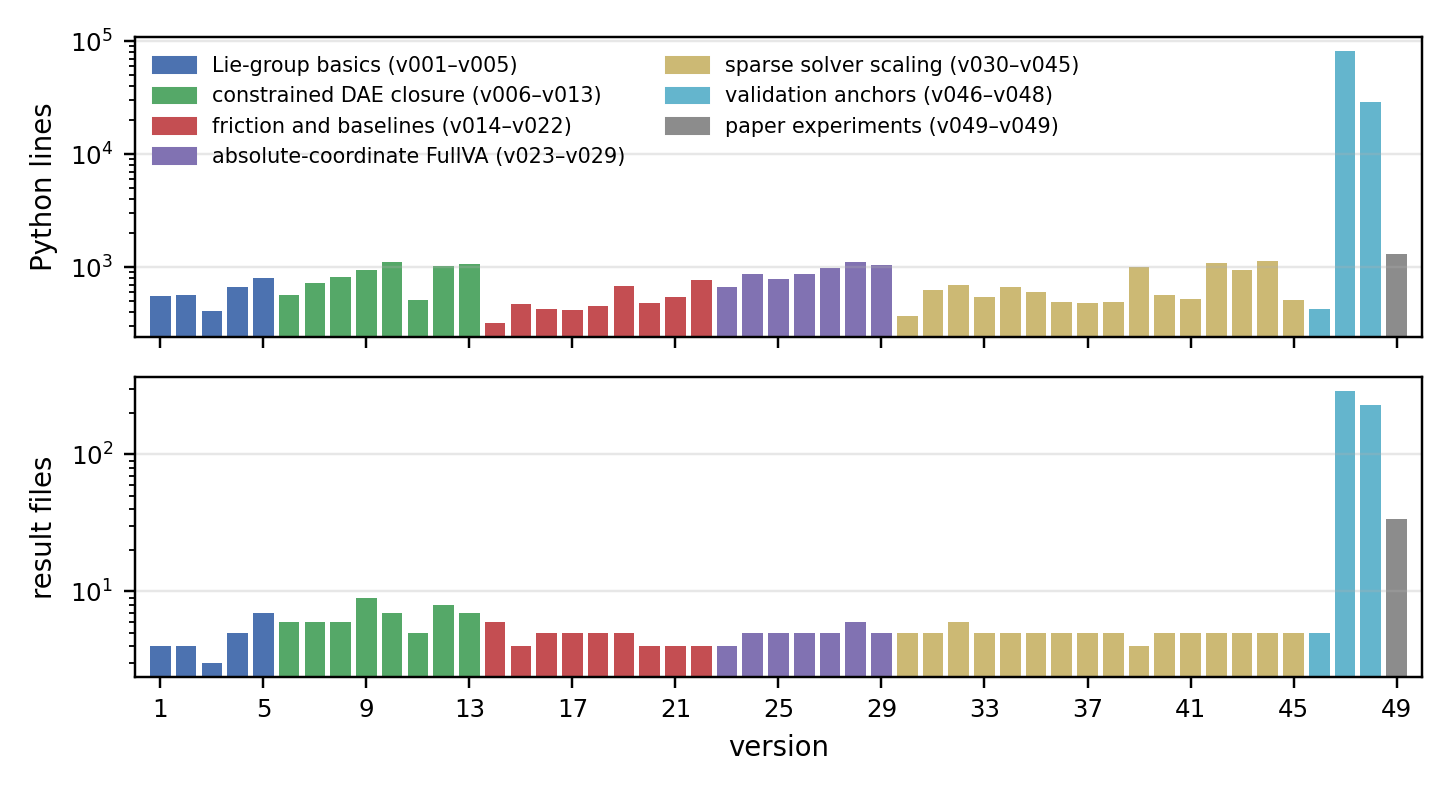
\includegraphics[width=0.92\textwidth]{figures/fig_versions.png}
  \caption{The 49 versioned experiments, coloured by phase, with the size of their code and the
  number of result files each left behind. The exploratory burst v001--v048 was produced in about three weeks in late May and early June 2026;
  v046--v048 (validation anchors) and v049 (paper experiments) carry the bulk of the artefacts.}
  \label{fig:versions}
\end{figure*}

Appendix~\ref{app:ledger} condenses the exploration into phases (Table~\ref{tab:phases}) and lists
every version (Table~\ref{tab:ledger}). In outline: Lie-group basics and the choice of Gauss
collocation (v001--v005); constrained DAE closure in absolute coordinates, friction, automatic
differentiation and quaternions (v006--v013); friction regimes and the rejection of trapezoidal, BDF
and Lobatto baselines (v014--v022); the absolute-coordinate revolute DAE and the emergence of the
FullVA stage system (v023--v029); sixteen versions of sparse-solver work (v030--v045); validation
anchors (v046--v048); and the experiments of the rewritten paper (v049). Three features of the
trajectory matter for the argument of this paper.


\paragraph{Negative results were the steering signal}
Of the 48 exploratory versions, about twenty exist to rule something out. The pattern that produced the
method is v023--v029: a full absolute-coordinate revolute DAE (v023) showed endpoint
velocity-level constraint drift; swapping Gauss nodes for Lobatto (v024) did not remove it;
projecting the endpoint after the step (v025) removed it but changed the method; adding the
velocity-level constraint rows at the stages (v026) and then the acceleration-level rows (v027)
removed it without changing the method. The last of these is the FullVA stage system. Its
generalization to a second joint (v029) and to non-revolute pairs (v043--v044) then tested that
the construction was not specific to one mechanism. Without the preserved negative results the
same agent, in a later session, would have retried the projection repair; the memory of why it was
wrong is what the versioned tree stores.

\paragraph{Sixteen versions of solver work produced no paper result, and that is recorded}
v030--v045 investigated sparse Jacobians for the growing stage systems. The sparse structure was
found, coloured and cached correctly, and dense automatic differentiation remained faster on every
problem tried. The ledger records ``sparse structure verified'' and forbids ``sparse speed
superiority''; the companion paper says one sentence about it. An agent optimizing for a paper
would have dropped or dressed up this phase; the ledger made the honest outcome the cheap one.

\paragraph{The theorem came from an audit, not from a search}
By September the manuscript displayed the stage system as body-level collocation rows, while the
code solved joint-coordinate collocation rows together with the full constraint hierarchy. The
agent was asked to reconcile the two. Working through the row inventory it found that the
$132$-row residual is zero at the lifted reduced Gauss stage, that the converse holds on the
regular branch, and hence that the implemented method \emph{is} reduced Gauss collocation in
disguise. This replaced what had been a conditional order argument with an open stage-residual
hypothesis by an exact identity plus two explicit perturbations, and it made the sixth order a
consequence of classical theory rather than a conjecture supported by slopes. The Lean development
was started the same day to check the identity row by row; the two hypotheses that the earlier
argument had kept as assumptions were then derived from smoothness. The discovery was not the
agent proposing a new idea. It was the agent being required to make two descriptions of the same
object agree, and refusing to paper over the difference.

\paragraph{The rewrite}
The manuscript that the ledger had grown around was 13\,000 lines, then 4\,000 after a
compaction, and read as a catalogue of what was not claimed. The human judged it poor. The agent
proposed a full rewrite with a new experiment set, delivered an outline, an experiment plan with
costs and an introduction for review, and after approval executed it: seven experiments, three
schematic figures, a 44-page manuscript with its arXiv and flat copies, and the new validator, in
about four days with \nHuman{} human messages (Section~\ref{sec:quant}).
